\documentclass[a4paper, 10pt]{article}

\usepackage{amsmath}
\usepackage{amssymb}
\usepackage{booktabs}
\usepackage[margin=1in]{geometry}
\usepackage{graphicx}
\usepackage{kotex}
\usepackage{float}
\usepackage{setspace}

\usepackage{enumitem}
\setlist[itemize]{nosep}
\setlist[enumerate]{nosep}


\begin{document}
    \onehalfspacing

    \section{Data Clearing}
        \begin{itemize}
            \item 서울, 경기, 인천, 제주를 제외하고 사용된 총 지역 수 - 160개 시군구
            \item 서울, 경기, 인천, 제주를 포함하는 총 지역 수 - 239개 시군구
            \item 지역 통합 규칙
                \begin{itemize}
                    \item 경북 군위군 (07-24), 대구 군위군 (2025) \\
                        $\Rightarrow$ 경북 군위군으로 통합
                    \item 인천 남구 (07-18), 인천 미추홀구 (19-25) \\
                        $\Rightarrow$ 인천 남구로 통합
                    \item 경기 부천시 (17-23), 경기 부천시 소사구\&오정구\&원미구 (07-16, 24-25) \\
                        $\Rightarrow$ 경기 부천시로 통합
                    \item 세종 세종시 (13-), 충북 청원군 (07-14), 충북 청주시 청원구\&서원구(15-25),
                        충북 청주시 상당구\&흥덕구 (07-25), 충남 연기군 (07-12), 충남 공주시 (07-25) \\
                        $\Rightarrow$ 삭제 (세종이 들어오면서 경계가 변화하였거나 세종시에 흡수된 지역)
                    \item 충남 천안시(07-08), 충남 천안시 서북구\&동남구 (10-25) \\
                        $\Rightarrow$ 충남 천안시로 통합
                    \item 경남 마산시\&진해시\&창원시 (07-12),
                        경남 창원시 마산합포구\&진해구\&의창구\&성산구(13-25) \\
                        $\Rightarrow$ 경남 창원시로 통합
                \end{itemize}
            \item 기간 - 2007년부터 2025년까지 19개 년도
            \item 사용된 종속변수들
                \begin{itemize}
                    \item 상급종합병원, 종합병원, 병원, 의원 개수
                    \item 인턴, 레지던트, 전문의, 일반의 명수
                \end{itemize}
            \item 사용된 독립변수들
                \begin{itemize}
                    \item Travel time
                \end{itemize}
            \item Travel time의 정의
                \begin{itemize}
                    \item Region $i$의 year $t$에서 서울 용산역 travel time을
                        $Tr_{it}$로 정의
                    \item $Tr_{it}$는 자동차만 이용하는 경우와 KTX를 이용하는 경우 중 더 짧은 시간으로 정의
                        \begin{align*}
                            Tr_{it}
                            &=
                            \min\{Tr^{car}_{it}, Tr^{KTX}_{it}\}.
                        \end{align*}
                    \item 자동차 경로는 시군구 centroid에서 용산역까지의 driving time
                        \begin{align*}
                            Tr^{car}_{it}
                            &=
                            Tr^{car}_{i,\text{centroid}\rightarrow\text{Seoul}}.
                        \end{align*}
                        자동차 소요시간은 OpenStreetMap의 2026년 4월 23일 스냅샷 기준으로
                        OSRM을 이용해 계산
                    \item KTX 경로는 region $i$의 centroid에서 30km 이내에 있는 KTX 역들의 집합 $H_i$ 중
                        총 소요시간이 가장 짧은 station을 선택
                        \begin{align*}
                            Tr^{KTX}_{it}
                            &=
                            \min_{h \in H_i}
                            \left\{
                                Tr^{car}_{i,\text{centroid}\rightarrow h}
                                +
                                WaitPenalty
                                +
                                Tr^{KTX}_{h\rightarrow\text{Seoul/Yongsan},t}
                            \right\}.
                        \end{align*}
                    \item $Tr^{car}_{i,\text{centroid}\rightarrow h}$: 시군구 centroid에서 KTX 역 $h$까지의
                        driving time
                    \item $WaitPenalty$: KTX 탑승 전 대기시간 penalty.
                        20-40분 사이의 적당한 값에 결과가 크게 달라지지 않아서 30분으로 설정
                    \item $Tr^{KTX}_{h\rightarrow\text{Seoul/Yongsan},t}$: KTX 역 $h$에서
                        서울역 또는 용산역까지의 train travel time. 코레일 정보공개청구로 획득한
                        KTX 시간표 데이터를 파싱하여 계산하며, 열차별 소요시간 차이를 고려해
                        median travel time을 사용
                \end{itemize}
        \end{itemize}

    \section{Travel Time 채택 이유}
        \begin{enumerate}
            \item 가장 큰 이유는
                기존의 threshold 거리 안에 KTX shock을 받은 역이 있는 경우에 treatment를
                받은 것으로 정의했던 기존의 방식이 결과가 잘 나오지 않았다.
            \item 테이블 \ref{tab:cutoff_sensitivity}에서 확인할 수 있듯 threshold를 어떻게 설정하느냐에 따라
                treatment를 받은 지역, 받지 않은 지역이 너무 크게크게 변했다.
            \item treatment를 받았다고 할 수 있을까 의문이 드는 지역에 기존 정의를 쓰면
                treatment를 받았다고 할 수 밖에 없는 상황에 놓인 경우도 있었다.
                일례로 경북 예천군이 있다. 경북 예천군은 주위에 영주역이 있고
                경북 예천군의 centroid와 영주역의 거리가 21km 정도여서 30km threshold 기준
                영주역에 KTX가 21년부터 다니기 시작하였으니
                treatment를 21년에 받았다고 정의되는 상황이었다. 그러나 경북 예천군 출신 과 동기가
                본가에 갈 때 단 한번도 KTX를 타고 가는 것을 보지 못해 무언가 이상하여 동기에게 물어본 결과
                버스를 타고 가나 KTX를 타고 가나 시간 면에서 큰 차이가 나지 않기도 하고 이미 시외버스를 잘 이용하고
                있으며 예천군의 주요 지역에서 영주역, 안동역 등 기차역에 가는 것 보다 예천터미널에 가는 것이
                접근성이 더 좋아서 사람들이 대체로 KTX를 잘 타지 않는다는 답변을 얻었다.
                위와 같은 상황을 기존의 방식이 잘 반영하지 못한다고 판단하였다.
            \item 그 외 호남선처럼 KTX가
                개통되어있긴 했는데 지속적으로 소요시간이 짧아진 경우,
                KTX가 운행하다가 노선 개편으로
                더이상 운행하지 않게 된 경우 등을 처리하기 위해 Travel time을 위와 같은
                방법으로 계산하였다.
        \end{enumerate}
        \begin{table}[H]
            \centering
            \caption{Treatment status by distance cutoff}
            \label{tab:cutoff_sensitivity}
            \begin{tabular}{rrrrr}
\toprule
Cutoff & Analysis regions & Treated & Control & Already treated\\
\midrule
10km & 132 & 29 & 103 & 28\\
20km & 122 & 44 & 78 & 38\\
30km & 110 & 62 & 48 & 50\\
40km & 96 & 68 & 28 & 64\\
50km & 84 & 72 & 12 & 76\\
\bottomrule
\end{tabular}

        \end{table}

    \section{분석}
    \subsection{사용 변수}
        병원 수 변수는
        $\log(hospital\_no+1)$로 변환하여 사용하였고 
        의사 수 변수는 $\log(doctor\_no+1)$로 변환하여 사용하였다.
        독립변수로는 $TravelTime$, $Saving$, $KTXWithin2h$를 사용하였다.
        $TravelTime$은 위의 정의와 동일하며 나머지 두 변수는
        다음과 같이 정의하였다.
        $Saving_{it}$는 2007년의 travel time을 기준으로 한 travel-time saving이다.
        \begin{align*}
            Saving_{it} = TravelTime_{i,2007} - TravelTime_{it}
        \end{align*}
        즉, $Saving_{it}$가 클수록 2007년 대비 terminal 접근시간이 더 많이 단축된
        지역-연도라는 뜻이다.
        $KTXWithin2h_{it}$는 KTX를 이용한 terminal 접근시간이
        2시간 이하이고, 동시에 자동차 travel time보다 짧은 경우 1을 갖는 더미변수이다.
        \begin{align*}
            KTXWithin2h_{it}
            =
            \mathbf{1}\{TravelTime^{KTX}_{it} \leq 2,\;
            TravelTime^{KTX}_{it} < TravelTime^{car}_{it}\}
        \end{align*}
        모든 회귀식에는 $\log(Population_{it})$ control, region fixed effects,
        year fixed effects를 포함하였고, standard error는 region level에서 cluster하였다.
        
    \subsection{회귀 결과}
        \subsubsection{Travel time}
        \begin{align*}
            Y_{it}
            =
            \alpha_i + \tau_t + \beta TravelTime_{it}
            + \gamma \log(Population_{it}) + \epsilon_{it}
        \end{align*}

        \begin{table}[H]
            \centering
            \caption{Travel Time: 의원}
            \input{meeting_tt_travel_time_hospital_clinic.tex}
        \end{table}

        \begin{table}[H]
            \centering
            \caption{Travel Time: 병원}
            \input{meeting_tt_travel_time_hospital_secondary.tex}
        \end{table}

        \begin{table}[H]
            \centering
            \caption{Travel Time: 종합병원}
            \input{meeting_tt_travel_time_hospital_general.tex}
        \end{table}

        \begin{table}[H]
            \centering
            \caption{Travel Time: 상급종합병원}
            \begingroup
\centering
\begin{tabular}{lcccccc}
   \toprule
                          & hospital\_no   & net\_entry  & exit\_no  & exit\_rate  & entry\_no  & entry\_rate \\    
                          & (1)            & (2)         & (3)       & (4)         & (5)        & (6)\\  
   \midrule 
   $TravelTime_{it}$      & -0.2213$^{**}$ & 0.0414      & -0.0105   & -0.0065     & 0.0265     & 0.1826\\   
                          & (0.0946)       & (0.0498)    & (0.0107)  & (0.0069)    & (0.0556)   & (0.1390)\\   
   Log population control & Yes            & Yes         & Yes       & Yes         & Yes        & Yes\\  
   Region FE              & Yes            & Yes         & Yes       & Yes         & Yes        & Yes\\  
   Year FE                & Yes            & Yes         & Yes       & Yes         & Yes        & Yes\\  
   Regions                & 20             & 20          & 20        & 20          & 20         & 20\\  
    \\
   Observations           & 380            & 360         & 380       & 279         & 360        & 266\\  
   Adjusted R$^2$         & 0.71399        & -0.04893    & -0.00220  & -0.01029    & -0.05670   & 0.06593\\  
   \bottomrule
\end{tabular}
\par\endgroup

        \end{table}

        \begin{table}[H]
            \centering
            \caption{Travel Time: 의사 수}
            \input{meeting_tt_travel_time_doctor.tex}
        \end{table}

        \subsubsection{Travel-time saving}
        \begin{align*}
            Y_{it}
            =
            \alpha_i + \tau_t + \beta Saving_{it}
            + \gamma \log(Population_{it}) + \epsilon_{it}
        \end{align*}

        \begin{table}[H]
            \centering
            \caption{Travel-Time Saving: 의원}
            \begingroup
\centering
\begin{tabular}{lcccccc}
   \toprule
                          & hospital\_no  & net\_entry    & exit\_no  & exit\_rate  & entry\_no  & entry\_rate \\    
                          & (1)           & (2)           & (3)       & (4)         & (5)        & (6)\\  
   \midrule 
   $Saving_{it}$          & -0.0147       & -0.3922$^{*}$ & -0.1147   & 0.0013      & -0.3868    & -0.0002\\   
                          & (0.0157)      & (0.2142)      & (0.2223)  & (0.0028)    & (0.2989)   & (0.0040)\\   
   Log population control & Yes           & Yes           & Yes       & Yes         & Yes        & Yes\\  
   Region FE              & Yes           & Yes           & Yes       & Yes         & Yes        & Yes\\  
   Year FE                & Yes           & Yes           & Yes       & Yes         & Yes        & Yes\\  
   Regions                & 159           & 159           & 159       & 159         & 159        & 159\\  
    \\
   Observations           & 3,021         & 2,862         & 3,021     & 3,021       & 2,862      & 2,862\\  
   Adjusted R$^2$         & 0.99410       & 0.33416       & 0.76165   & 0.14685     & 0.70929    & 0.06275\\  
   \bottomrule
\end{tabular}
\par\endgroup

        \end{table}

        \begin{table}[H]
            \centering
            \caption{Travel-Time Saving: 병원}
            \begingroup
\centering
\begin{tabular}{lcccccc}
   \toprule
                          & hospital\_no  & net\_entry  & exit\_no     & exit\_rate  & entry\_no  & entry\_rate \\    
                          & (1)           & (2)         & (3)          & (4)         & (5)        & (6)\\  
   \midrule 
   $Saving_{it}$          & 0.0728        & -0.0629     & 0.1305$^{*}$ & 0.0188      & 0.0577     & -0.0080\\   
                          & (0.0550)      & (0.1300)    & (0.0711)     & (0.0155)    & (0.1419)   & (0.0232)\\   
   Log population control & Yes           & Yes         & Yes          & Yes         & Yes        & Yes\\  
   Region FE              & Yes           & Yes         & Yes          & Yes         & Yes        & Yes\\  
   Year FE                & Yes           & Yes         & Yes          & Yes         & Yes        & Yes\\  
   Regions                & 151           & 151         & 151          & 151         & 151        & 151\\  
    \\
   Observations           & 2,869         & 2,718       & 2,869        & 2,730       & 2,718      & 2,587\\  
   Adjusted R$^2$         & 0.90271       & 0.06402     & 0.32401      & 0.04765     & 0.27994    & 0.05955\\  
   \bottomrule
\end{tabular}
\par\endgroup

        \end{table}

        \begin{table}[H]
            \centering
            \caption{Travel-Time Saving: 종합병원}
            \begingroup
\centering
\begin{tabular}{lcccccc}
   \toprule
                          & hospital\_no  & net\_entry  & exit\_no  & exit\_rate  & entry\_no  & entry\_rate \\    
                          & (1)           & (2)         & (3)       & (4)         & (5)        & (6)\\  
   \midrule 
   $Saving_{it}$          & -0.0096       & -0.0183     & -0.0308   & -0.0172     & -0.0379    & -0.0192\\   
                          & (0.0355)      & (0.0254)    & (0.0209)  & (0.0108)    & (0.0299)   & (0.0205)\\   
   Log population control & Yes           & Yes         & Yes       & Yes         & Yes        & Yes\\  
   Region FE              & Yes           & Yes         & Yes       & Yes         & Yes        & Yes\\  
   Year FE                & Yes           & Yes         & Yes       & Yes         & Yes        & Yes\\  
   Regions                & 99            & 99          & 99        & 99          & 99         & 99\\  
    \\
   Observations           & 1,881         & 1,782       & 1,881     & 1,678       & 1,782      & 1,594\\  
   Adjusted R$^2$         & 0.83074       & -0.01077    & 0.09022   & 0.05918     & 0.04723    & 0.05436\\  
   \bottomrule
\end{tabular}
\par\endgroup

        \end{table}

        \begin{table}[H]
            \centering
            \caption{Travel-Time Saving: 상급종합병원}
            \input{meeting_tt_saving_hospital_tertiary.tex}
        \end{table}

        \begin{table}[H]
            \centering
            \caption{Travel-Time Saving: 의사 수}
            \begingroup
\centering
\begin{tabular}{lcccc}
   \toprule
                          & 인턴     & 레지던트      & 전문의   & 일반의 \\   
                          & (1)      & (2)           & (3)      & (4)\\  
   \midrule 
   $Saving_{it}$          & -0.0472  & -0.2005$^{*}$ & 0.0078   & 0.0303\\   
                          & (0.0581) & (0.1141)      & (0.0257) & (0.0278)\\   
   Log population control & Yes      & Yes           & Yes      & Yes\\  
   Region FE              & Yes      & Yes           & Yes      & Yes\\  
   Year FE                & Yes      & Yes           & Yes      & Yes\\  
   Regions                & 160      & 160           & 160      & 160\\  
    \\
   Observations           & 3,040    & 3,040         & 3,040    & 3,040\\  
   Adjusted R$^2$         & 0.83484  & 0.92483       & 0.98982  & 0.86034\\  
   \bottomrule
\end{tabular}
\par\endgroup

        \end{table}

        \subsubsection{KTX within two hours}
        특이사항으로, $KTXWithin2h$ 변수에서 threshold 시간을 1.5, 2.5, 3, 3.5 등으로
        바꿔보아도 크게 유의미한 결과가 나오지 않았음
        \begin{align*}
            Y_{it}
            =
            \alpha_i + \tau_t + \delta KTXWithin2h_{it}
            + \gamma \log(Population_{it}) + \epsilon_{it}
        \end{align*}

        \begin{table}[H]
            \centering
            \caption{KTX Within Two Hours: 의원}
            \begingroup
\centering
\begin{tabular}{lcccccc}
   \toprule
                          & hospital\_no  & net\_entry  & exit\_no  & exit\_rate  & entry\_no     & entry\_rate \\    
                          & (1)           & (2)         & (3)       & (4)         & (5)           & (6)\\  
   \midrule 
   $KTXWithin2h_{it}$     & -0.0071       & 0.1728      & 0.2338    & 0.0033      & 0.5022$^{**}$ & 0.0004\\   
                          & (0.0265)      & (0.2421)    & (0.3006)  & (0.0047)    & (0.2367)      & (0.0085)\\   
   Log population control & Yes           & Yes         & Yes       & Yes         & Yes           & Yes\\  
   Region FE              & Yes           & Yes         & Yes       & Yes         & Yes           & Yes\\  
   Year FE                & Yes           & Yes         & Yes       & Yes         & Yes           & Yes\\  
   Regions                & 159           & 159         & 159       & 159         & 159           & 159\\  
    \\
   Observations           & 3,021         & 2,862       & 3,021     & 3,021       & 2,862         & 2,862\\  
   Adjusted R$^2$         & 0.99409       & 0.33352     & 0.76164   & 0.14686     & 0.70916       & 0.06275\\  
   \bottomrule
\end{tabular}
\par\endgroup

        \end{table}

        \begin{table}[H]
            \centering
            \caption{KTX Within Two Hours: 병원}
            \begingroup
\centering
\begin{tabular}{lcccccc}
   \toprule
                          & hospital\_no  & net\_entry  & exit\_no  & exit\_rate  & entry\_no  & entry\_rate \\    
                          & (1)           & (2)         & (3)       & (4)         & (5)        & (6)\\  
   \midrule 
   $KTXWithin2h_{it}$     & 0.1703        & 0.1489      & 0.0279    & 0.0135      & 0.1606     & -0.0104\\   
                          & (0.1149)      & (0.1815)    & (0.0465)  & (0.0247)    & (0.1970)   & (0.0540)\\   
   Log population control & Yes           & Yes         & Yes       & Yes         & Yes        & Yes\\  
   Region FE              & Yes           & Yes         & Yes       & Yes         & Yes        & Yes\\  
   Year FE                & Yes           & Yes         & Yes       & Yes         & Yes        & Yes\\  
   Regions                & 151           & 151         & 151       & 151         & 151        & 151\\  
    \\
   Observations           & 2,869         & 2,718       & 2,869     & 2,730       & 2,718      & 2,587\\  
   Adjusted R$^2$         & 0.90274       & 0.06405     & 0.32291   & 0.04735     & 0.28000    & 0.05952\\  
   \bottomrule
\end{tabular}
\par\endgroup

        \end{table}

        \begin{table}[H]
            \centering
            \caption{KTX Within Two Hours: 종합병원}
            \begingroup
\centering
\begin{tabular}{lcccccc}
   \toprule
                          & hospital\_no  & net\_entry  & exit\_no  & exit\_rate  & entry\_no  & entry\_rate \\    
                          & (1)           & (2)         & (3)       & (4)         & (5)        & (6)\\  
   \midrule 
   $KTXWithin2h_{it}$     & -0.0622       & -0.0245     & -0.0367   & -0.0359     & -0.0589    & -0.0492\\   
                          & (0.0577)      & (0.0306)    & (0.0242)  & (0.0273)    & (0.0372)   & (0.0358)\\   
   Log population control & Yes           & Yes         & Yes       & Yes         & Yes        & Yes\\  
   Region FE              & Yes           & Yes         & Yes       & Yes         & Yes        & Yes\\  
   Year FE                & Yes           & Yes         & Yes       & Yes         & Yes        & Yes\\  
   Regions                & 99            & 99          & 99        & 99          & 99         & 99\\  
    \\
   Observations           & 1,881         & 1,782       & 1,881     & 1,678       & 1,782      & 1,594\\  
   Adjusted R$^2$         & 0.83085       & -0.01100    & 0.08936   & 0.05870     & 0.04667    & 0.05422\\  
   \bottomrule
\end{tabular}
\par\endgroup

        \end{table}

        \begin{table}[H]
            \centering
            \caption{KTX Within Two Hours: 상급종합병원}
            \begingroup
\centering
\begin{tabular}{lcccccc}
   \toprule
                          & hospital\_no  & net\_entry     & exit\_no       & exit\_rate     & entry\_no      & entry\_rate \\    
                          & (1)           & (2)            & (3)            & (4)            & (5)            & (6)\\  
   \midrule 
   $KTXWithin2h_{it}$     & 0.1113        & 0.0824$^{***}$ & 0.3332$^{***}$ & 0.1661$^{***}$ & 0.4155$^{***}$ & 0.2435$^{***}$\\   
                          & (0.0772)      & (0.0135)       & (0.0004)       & (0.0004)       & (0.0141)       & (0.0415)\\   
   Log population control & Yes           & Yes            & Yes            & Yes            & Yes            & Yes\\  
   Region FE              & Yes           & Yes            & Yes            & Yes            & Yes            & Yes\\  
   Year FE                & Yes           & Yes            & Yes            & Yes            & Yes            & Yes\\  
   Regions                & 20            & 20             & 20             & 20             & 20             & 20\\  
    \\
   Observations           & 380           & 360            & 380            & 279            & 360            & 266\\  
   Adjusted R$^2$         & 0.70095       & -0.04942       & 0.29216        & 0.28181        & -0.03081       & 0.06451\\  
   \bottomrule
\end{tabular}
\par\endgroup

        \end{table}

        \begin{table}[H]
            \centering
            \caption{KTX Within Two Hours: 의사 수}
            \begingroup
\centering
\begin{tabular}{lcccc}
   \toprule
                          & 인턴     & 레지던트 & 전문의   & 일반의 \\   
                          & (1)      & (2)      & (3)      & (4)\\  
   \midrule 
   $KTXWithin2h_{it}$     & 0.0611   & 0.0700   & 0.0220   & 0.0281\\   
                          & (0.0475) & (0.0709) & (0.0759) & (0.0655)\\   
   Log population control & Yes      & Yes      & Yes      & Yes\\  
   Region FE              & Yes      & Yes      & Yes      & Yes\\  
   Year FE                & Yes      & Yes      & Yes      & Yes\\  
   Regions                & 160      & 160      & 160      & 160\\  
    \\
   Observations           & 3,040    & 3,040    & 3,040    & 3,040\\  
   Adjusted R$^2$         & 0.83479  & 0.92418  & 0.98982  & 0.86024\\  
   \bottomrule
\end{tabular}
\par\endgroup

        \end{table}
        
        \begin{figure}[H]
            \centering
            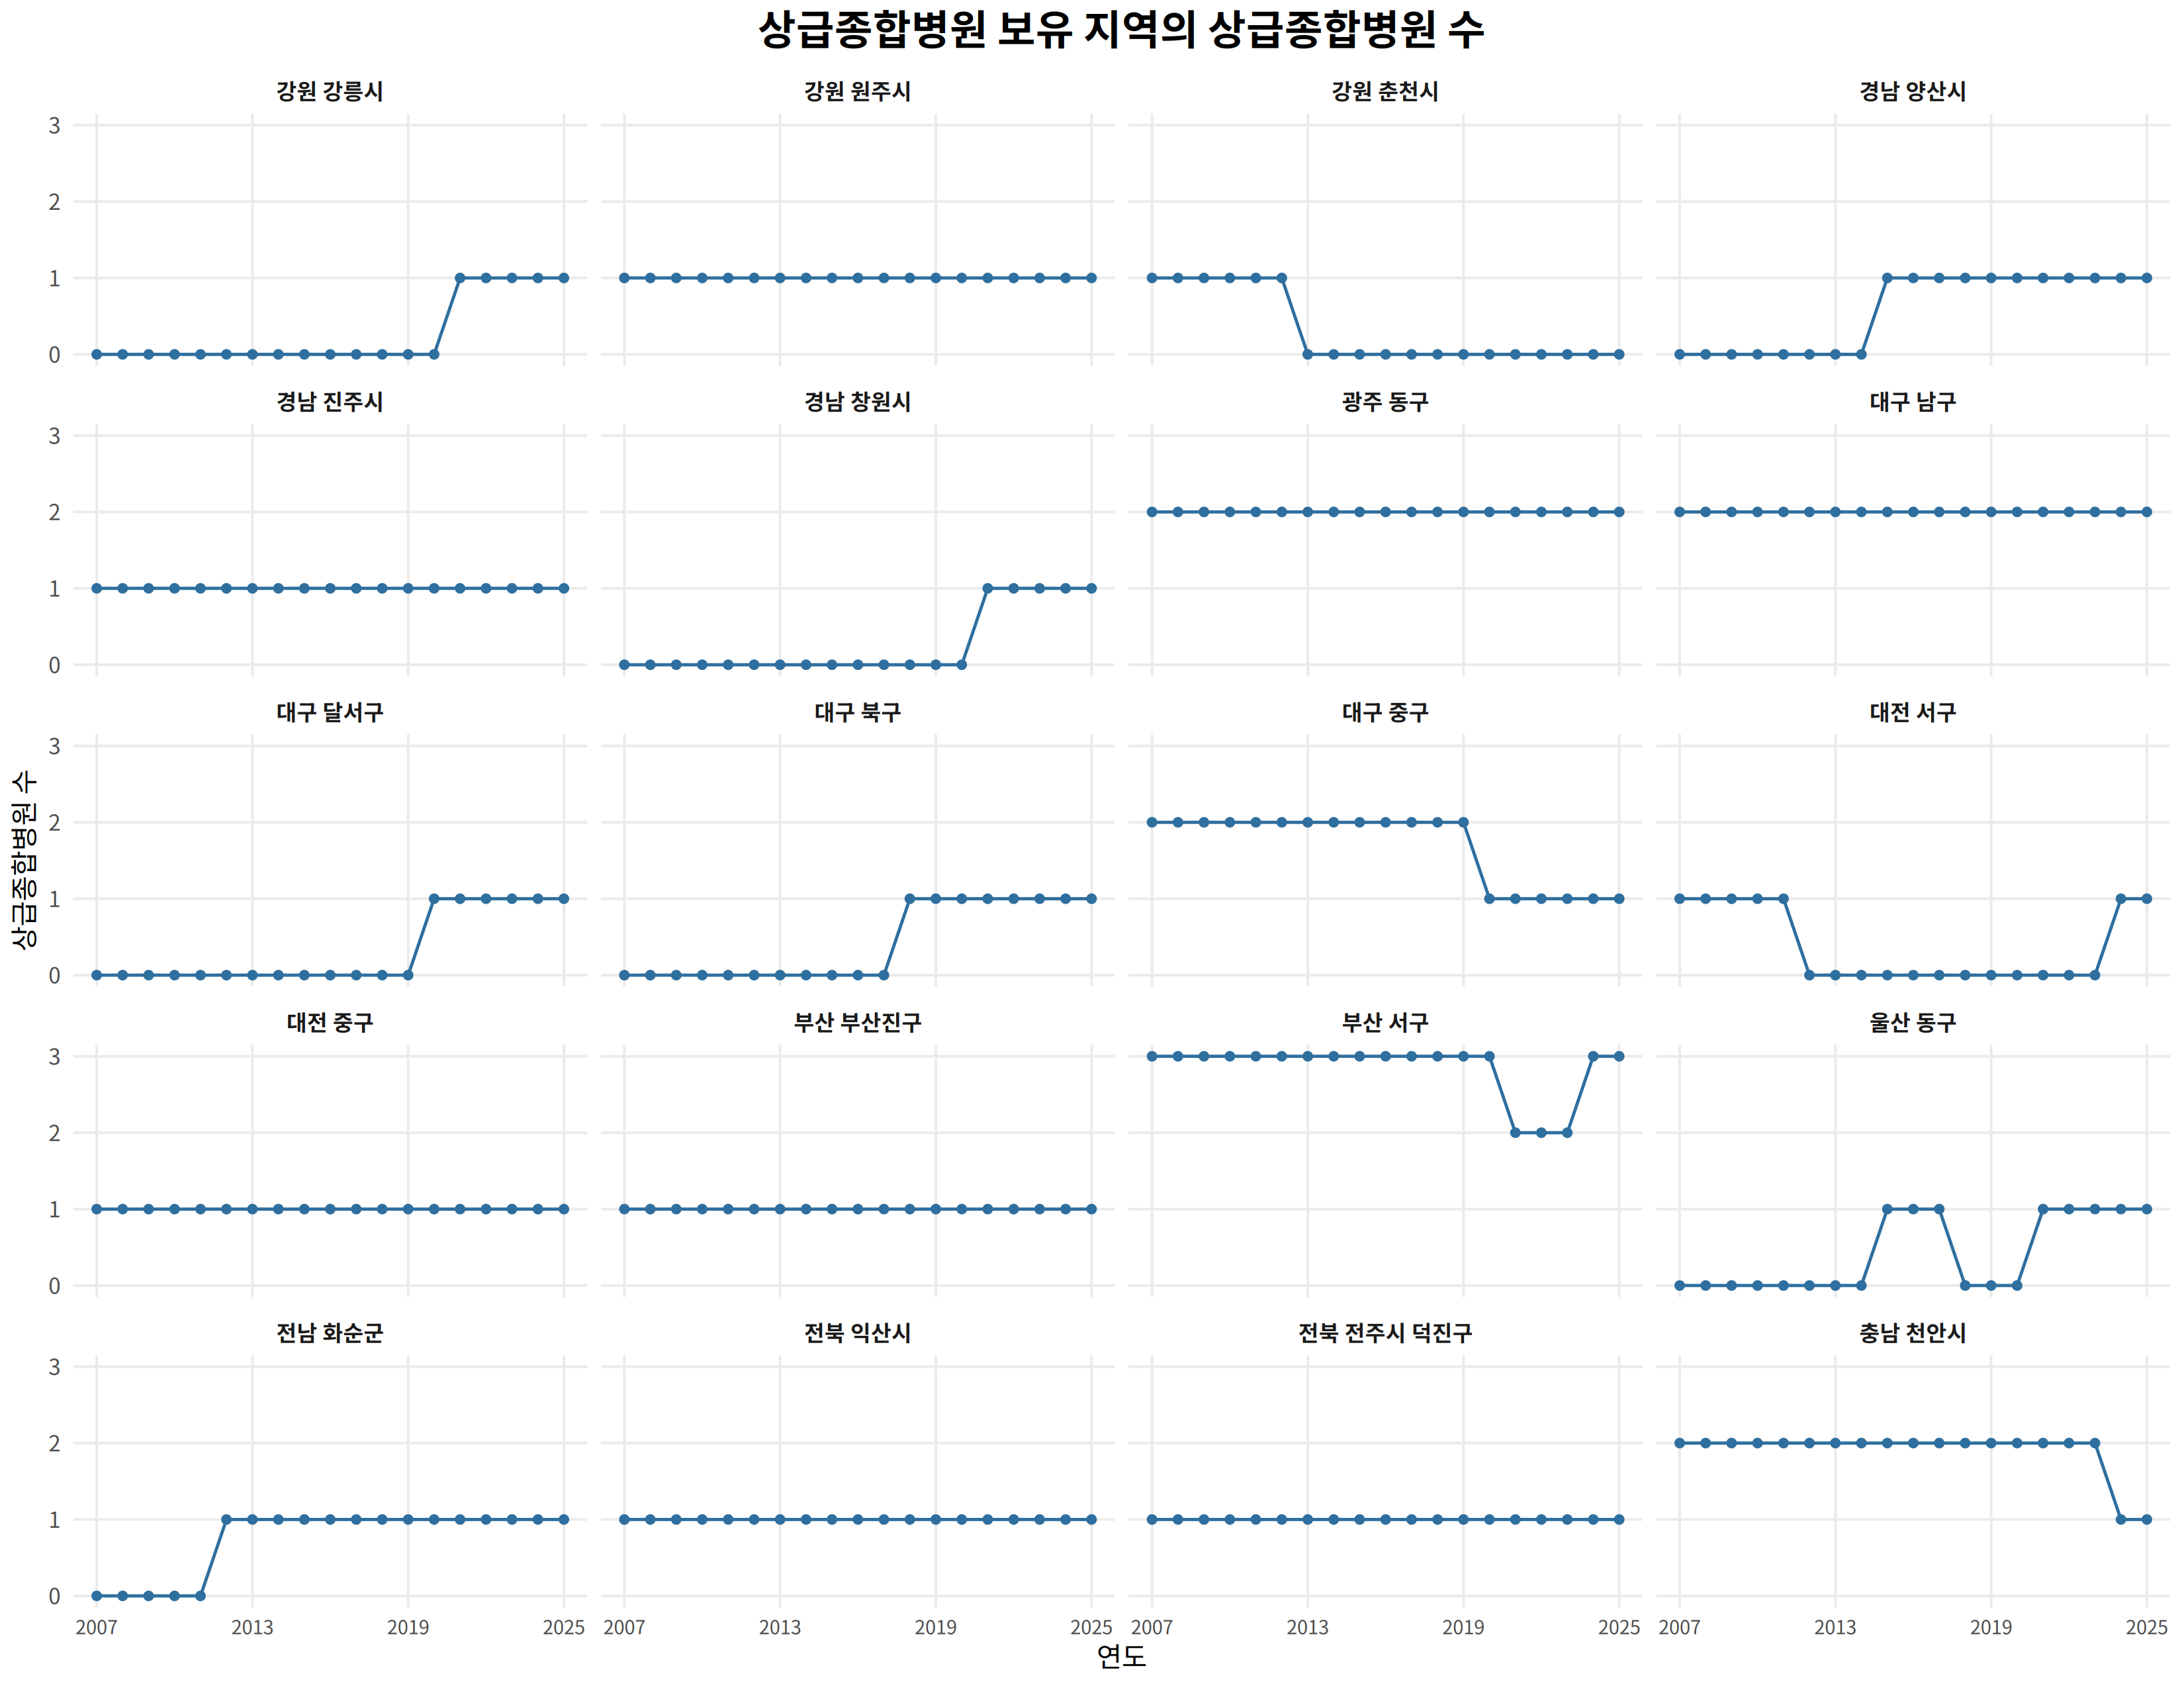
\includegraphics[width=\textwidth]{tertiary_hospital_count_by_region.png}
        \end{figure}
            

    
    \newpage
    \appendix
    
    \section{기존 shock 정의 분석결과}
        Shock은 시군구 centroid에서 30km 이내에 KTX 정차역이 존재하는 경우로 정의하며,
        분석기간은 2007년부터 2025년까지이다. 모든 분석에서 서울, 경기, 인천, 제주는 제외하였다.
        병원 분석의 type별 표본은 해당 type 병원이 분석기간 전체에서 한 번도 관측되지 않는 지역을 제외하였다.
        의사 분석은 별도의 zero restriction 없이 서울, 경기, 인천, 제주를 제외한 지역 전체를 사용하였다.

        Rate 변수의 observation 수는 count 변수와 다를 수 있다.
        Entry rate와 exit rate는 해당 지역-연도에서 병원 수가 양수일 때만 정의되기 때문이다.
        Callaway and Sant'Anna simple ATT는 병원 분석의 경우 TWFE와 동일한 6개 종속변수에 대해 추정하였고,
        의사 분석의 경우 level별 의사 수를 사용하였다.
        또한 2007년 이전 또는 2007년에 이미 treated인 지역은
        회귀에 사용하지 않았다.

        \subsection{Summary Statistics}
            \begin{table}[H]
                \centering
                \caption{30km summary statistics: doctor sample}
                \input{meeting_summary_stats_doctor.tex}
            \end{table}

        \subsection{TWFE DiD}
            TWFE 분석은 다음 회귀식으로 추정하였다.
            Region fixed effects와 year fixed effects를 포함하고,
            standard error는 region level에서 cluster하였다.
            \begin{align*}
                Y_{it}
                &=
                \alpha_i
                +
                \lambda_t
                +
                \beta Shock_{it}
                +
                \varepsilon_{it}.
            \end{align*}

            \begin{table}[H]
                \centering
                \caption{TWFE DiD 의원}
                \begingroup
\centering
\begin{tabular}{lcccccc}
   \toprule
                        & hospital\_no  & net\_entry    & exit\_no        & exit\_rate    & entry\_no     & entry\_rate\\   
                        & (1)           & (2)           & (3)             & (4)           & (5)           & (6)\\  
   \midrule 
   $\beta$              & 2.604$^{*}$   & 0.2563        & -0.5022$^{***}$ & -0.0046       & -0.1297       & -0.0019\\   
                        & (1.518)       & (0.1936)      & (0.1530)        & (0.0046)      & (0.1986)      & (0.0057)\\   
    \\
   Region count         & 109           & 109           & 109           & 109           & 109           & 109\\
   Observations         & 2,071         & 1,962         & 2,071           & 2,071         & 1,962         & 1,962\\  
   R$^2$                & 0.99215       & 0.26686       & 0.75411         & 0.18310       & 0.67742       & 0.11067\\  
    \\
   region fixed effects & $\checkmark$  & $\checkmark$  & $\checkmark$    & $\checkmark$  & $\checkmark$  & $\checkmark$\\   
   year fixed effects   & $\checkmark$  & $\checkmark$  & $\checkmark$    & $\checkmark$  & $\checkmark$  & $\checkmark$\\   
   \bottomrule
\end{tabular}
\par\endgroup

            \end{table}

            \begin{table}[H]
                \centering
                \caption{TWFE DiD 병원}
                \begingroup
\centering
\begin{tabular}{lcccccc}
   \toprule
                        & hospital\_no  & net\_entry     & exit\_no      & exit\_rate    & entry\_no     & entry\_rate\\   
                        & (1)           & (2)            & (3)           & (4)           & (5)           & (6)\\  
   \midrule 
   $\beta$              & 0.5154$^{*}$  & -0.1516$^{**}$ & 0.1401$^{**}$ & 0.0173        & -0.0011       & 0.0019\\   
                        & (0.2918)      & (0.0763)       & (0.0675)      & (0.0208)      & (0.0850)      & (0.0224)\\   
    \\
   Region count         & 102           & 102           & 102           & 102           & 102           & 102\\
   Observations         & 1,938         & 1,836          & 1,938         & 1,811         & 1,836         & 1,715\\  
   R$^2$                & 0.94258       & 0.14445        & 0.39280       & 0.11635       & 0.38288       & 0.12300\\  
    \\
   region fixed effects & $\checkmark$  & $\checkmark$   & $\checkmark$  & $\checkmark$  & $\checkmark$  & $\checkmark$\\   
   year fixed effects   & $\checkmark$  & $\checkmark$   & $\checkmark$  & $\checkmark$  & $\checkmark$  & $\checkmark$\\   
   \bottomrule
\end{tabular}
\par\endgroup

            \end{table}

            \begin{table}[H]
                \centering
                \caption{TWFE DiD 종합병원}
                \begingroup
\centering
\begin{tabular}{lcccccc}
   \toprule
                        & hospital\_no  & net\_entry    & exit\_no              & exit\_rate    & entry\_no     & entry\_rate\\   
                        & (1)           & (2)           & (3)                   & (4)           & (5)           & (6)\\  
   \midrule 
   $\beta$              & 0.0503        & -0.0381       & $6.37\times 10^{-5}$  & -0.0003       & -0.0311       & -0.0082\\   
                        & (0.0898)      & (0.0309)      & (0.0234)              & (0.0118)      & (0.0374)      & (0.0222)\\   
    \\
   Region count         & 59           & 59           & 59           & 59           & 59           & 59\\
   Observations         & 1,121         & 1,062         & 1,121                 & 997           & 1,062         & 948\\  
   R$^2$                & 0.94512       & 0.07017       & 0.16047               & 0.11280       & 0.13978       & 0.12761\\  
    \\
   region fixed effects & $\checkmark$  & $\checkmark$  & $\checkmark$          & $\checkmark$  & $\checkmark$  & $\checkmark$\\   
   year fixed effects   & $\checkmark$  & $\checkmark$  & $\checkmark$          & $\checkmark$  & $\checkmark$  & $\checkmark$\\   
   \bottomrule
\end{tabular}
\par\endgroup

            \end{table}

            \begin{table}[H]
                \centering
                \caption{TWFE DiD 상급종합병원}
                % Skipped outcomes: exit_no, exit_rate
\begingroup
\centering
\begin{tabular}{lcccc}
   \toprule
                        & hospital\_no  & net\_entry    & entry\_no     & entry\_rate\\   
                        & (1)           & (2)           & (3)           & (4)\\  
   \midrule 
   $\beta$              & 0.3548        & -0.0317       & -0.0317       & 0.0019\\   
                        & (0.3168)      & (0.0592)      & (0.0592)      & (0.0341)\\   
    \\
   Region count         & 8           & 8           & 8           & 8\\
   Observations         & 152           & 144           & 144           & 91\\  
   R$^2$                & 0.78558       & 0.25843       & 0.25843       & 0.46064\\  
    \\
   region fixed effects & $\checkmark$  & $\checkmark$  & $\checkmark$  & $\checkmark$\\   
   year fixed effects   & $\checkmark$  & $\checkmark$  & $\checkmark$  & $\checkmark$\\   
   \bottomrule
\end{tabular}
\par\endgroup

            \end{table}

            \begin{table}[H]
                \centering
                \caption{TWFE DiD 의사 수}
                \begingroup
\centering
\begin{tabular}{lcccc}
   \toprule
                        & intern        & resident      & specialist    & general\_doctor\\   
                        & (1)           & (2)           & (3)           & (4)\\  
   \midrule 
   $\beta$              & -0.5451       & -3.245$^{**}$ & 27.40$^{***}$ & 0.2900\\   
                        & (0.3591)      & (1.601)       & (7.215)       & (0.6601)\\   
    \\
   Region count         & 110           & 110           & 110           & 110\\
   Observations         & 2,090         & 2,090         & 2,090         & 2,090\\  
   R$^2$                & 0.82719       & 0.93251       & 0.97360       & 0.87034\\  
    \\
   region fixed effects & $\checkmark$  & $\checkmark$  & $\checkmark$  & $\checkmark$\\   
   year fixed effects   & $\checkmark$  & $\checkmark$  & $\checkmark$  & $\checkmark$\\   
   \bottomrule
\end{tabular}
\par\endgroup

            \end{table}

        \subsection{Callaway and Sant'Anna Simple ATT}
            Callaway and Sant'Anna 방식의
            group-time ATT를 먼저 추정한 뒤, simple aggregation을 사용하였다.
            Control group은 not-yet-treated regions로 두었다.

            \begin{table}[H]
                \centering
                \caption{Callaway and Sant'Anna simple ATT 의원}
                
\begin{tabular}{lcccccc}
\toprule
 & hospital\_no & net\_entry & exit\_no & exit\_rate & entry\_no & entry\_rate\\
\midrule
$ATT$ & 4.680*** & 0.140 & -0.299 & 0.001 & -0.159 & 0.003\\
 & (1.751) & (0.401) & (0.297) & (0.007) & (0.483) & (0.010)\\
\midrule
Region count & 109 & 109 & 109 & 109 & 109 & 109\\
Observations & 2,071 & 1,962 & 2,071 & 2,071 & 1,962 & 1,962\\
\bottomrule
\end{tabular}

            \end{table}

            \begin{table}[H]
                \centering
                \caption{Callaway and Sant'Anna simple ATT 병원}
                
\begin{tabular}{lcccccc}
\toprule
 & hospital\_no & net\_entry & exit\_no & exit\_rate & entry\_no & entry\_rate\\
\midrule
$ATT$ & 0.298 & -0.132 & 0.203* & 0.052** & 0.070 & 0.014\\
 & (0.281) & (0.117) & (0.112) & (0.026) & (0.181) & (0.031)\\
\midrule
Region count & 102 & 102 & 102 & 102 & 102 & 102\\
Observations & 1,938 & 1,836 & 1,938 & 1,811 & 1,836 & 1,715\\
\bottomrule
\end{tabular}

            \end{table}

            \begin{table}[H]
                \centering
                \caption{Callaway and Sant'Anna simple ATT 종합병원}
                
\begin{tabular}{lcccccc}
\toprule
 & hospital\_no & net\_entry & exit\_no & exit\_rate & entry\_no & entry\_rate\\
\midrule
$ATT$ & 0.054 & -0.007 & -0.026 & 0.012 & -0.033 & 0.027\\
 & (0.113) & (0.059) & (0.063) & (0.024) & (0.094) & (0.031)\\
\midrule
Region count & 59 & 59 & 59 & 59 & 59 & 59\\
Observations & 1,121 & 1,062 & 1,121 & 997 & 1,062 & 949\\
\bottomrule
\end{tabular}

            \end{table}

            \begin{table}[H]
                \centering
                \caption{Callaway and Sant'Anna simple ATT 상급종합병원}
                
\begin{tabular}{lcccccc}
\toprule
 & hospital\_no & net\_entry & exit\_no & exit\_rate & entry\_no & entry\_rate\\
\midrule
$ATT$ & 0.556* & 0.045* & 0.000 & 0.000 & 0.045 & 0.061\\
 & (0.334) & (0.023) & (0.000) & (0.000) & (0.031) & (0.233)\\
\midrule
Region count & 8 & 8 & 8 & 8 & 8 & 8\\
Observations & 152 & 144 & 152 & 95 & 144 & 91\\
\bottomrule
\end{tabular}

            \end{table}

            \begin{table}[H]
                \centering
                \caption{Callaway and Sant'Anna simple ATT 의사}
                
\begin{tabular}{lcccc}
\toprule
 & intern & resident & specialist & general\_doctor\\
\midrule
$ATT$ & 0.733 & -2.029 & 30.358*** & 0.588\\
 & (0.871) & (1.842) & (8.854) & (0.575)\\
\midrule
Region count & 110 & 110 & 110 & 110\\
Observations & 2,090 & 2,090 & 2,090 & 2,090\\
\bottomrule
\end{tabular}

            \end{table}
        
        \subsection{Event Study}
            \begin{table}[H]
                \centering
                \caption{Event Study: 의원}
                \begingroup
\centering
\begin{tabular}{lcccccc}
   \toprule
                          & hospital\_no  & net\_entry   & exit\_no      & exit\_rate  & entry\_no  & entry\_rate \\    
                          & (1)           & (2)          & (3)           & (4)         & (5)        & (6)\\  
   \midrule 
   $t \leq -5$            & -0.9219       & -0.4560      & 0.2682        & 0.0024      & -0.2498    & -0.0067\\   
                          & (1.708)       & (0.4315)     & (0.3242)      & (0.0066)    & (0.5353)   & (0.0098)\\   
   $t = -4$               & 0.2335        & -0.5982      & 1.080$^{***}$ & 0.0145      & 0.1322     & -0.0052\\   
                          & (0.7281)      & (0.4357)     & (0.3471)      & (0.0095)    & (0.4907)   & (0.0137)\\   
   $t = -3$               & 0.2041        & -0.5917      & 0.0836        & 0.0028      & -0.4974    & -0.0007\\   
                          & (0.6805)      & (0.6847)     & (0.3390)      & (0.0099)    & (0.8015)   & (0.0138)\\   
   $t = -2$               & -0.1158       & -1.079$^{*}$ & 0.1239        & 0.0004      & -0.9364    & -0.0219\\   
                          & (0.6372)      & (0.5581)     & (0.3542)      & (0.0089)    & (0.6757)   & (0.0171)\\   
   $t = 0$                & 0.4139        & -0.3755      & -0.1790       & -0.0030     & -0.5464    & -0.0122\\   
                          & (0.4172)      & (0.4919)     & (0.2834)      & (0.0078)    & (0.5672)   & (0.0120)\\   
   $t = 1$                & 0.6702        & -0.4727      & 0.1798        & -0.0003     & -0.2735    & -0.0086\\   
                          & (0.5926)      & (0.4854)     & (0.3080)      & (0.0081)    & (0.5782)   & (0.0111)\\   
   $t = 2$                & 0.9685        & -0.4509      & 0.1852        & 0.0057      & -0.2522    & -0.0061\\   
                          & (0.8209)      & (0.5576)     & (0.3029)      & (0.0078)    & (0.5918)   & (0.0109)\\   
   $t = 3$                & 1.324         & -0.3314      & -0.3442       & -0.0036     & -0.6555    & -0.0120\\   
                          & (0.9643)      & (0.4371)     & (0.3132)      & (0.0085)    & (0.5369)   & (0.0124)\\   
   $t = 4$                & 1.634         & -0.3806      & -0.6294$^{*}$ & -0.0046     & -0.9889    & -0.0159\\   
                          & (1.143)       & (0.5134)     & (0.3346)      & (0.0078)    & (0.6117)   & (0.0109)\\   
   $t \geq 5$             & 5.765$^{***}$ & 0.0732       & -0.4454       & -0.0012     & -0.3460    & -0.0041\\   
                          & (2.083)       & (0.3852)     & (0.3095)      & (0.0067)    & (0.4753)   & (0.0101)\\   
   Log population control & Yes           & Yes          & Yes           & Yes         & Yes        & Yes\\  
   Region FE              & Yes           & Yes          & Yes           & Yes         & Yes        & Yes\\  
   Year FE                & Yes           & Yes          & Yes           & Yes         & Yes        & Yes\\  
   Regions                & 109           & 109          & 109           & 109         & 109        & 109\\  
    \\
   Observations           & 2,071         & 1,962        & 2,071         & 2,071       & 1,962      & 1,962\\  
   R$^2$                  & 0.99240       & 0.27246      & 0.75819       & 0.18519     & 0.67916    & 0.11287\\  
   \bottomrule
\end{tabular}
\par\endgroup

            \end{table}

            \begin{table}[H]
                \centering
                \caption{Event Study: 병원}
                \begingroup
\centering
\begin{tabular}{lcccccc}
   \toprule
                          & hospital\_no  & net\_entry  & exit\_no      & exit\_rate   & entry\_no  & entry\_rate \\    
                          & (1)           & (2)         & (3)           & (4)          & (5)        & (6)\\  
   \midrule 
   $t \leq -5$            & -0.6379$^{*}$ & 0.1467      & 0.0047        & 0.0097       & 0.1344     & -0.0140\\   
                          & (0.3585)      & (0.1520)    & (0.1162)      & (0.0354)     & (0.2202)   & (0.0431)\\   
   $t = -4$               & -0.3713       & 0.1160      & -0.0613       & -0.0162      & 0.0438     & 0.0295\\   
                          & (0.2724)      & (0.2125)    & (0.1392)      & (0.0341)     & (0.2536)   & (0.0486)\\   
   $t = -3$               & -0.0573       & 0.2304      & -0.0307       & -0.0063      & 0.1933     & 0.0232\\   
                          & (0.1937)      & (0.1644)    & (0.1425)      & (0.0417)     & (0.2126)   & (0.0510)\\   
   $t = -2$               & -0.0495       & -0.0982     & 0.2023        & 0.0460       & 0.0981     & -0.0163\\   
                          & (0.0999)      & (0.1505)    & (0.1264)      & (0.0364)     & (0.1885)   & (0.0582)\\   
   $t = 0$                & -0.0062       & -0.1166     & 0.3594$^{**}$ & 0.0675$^{*}$ & 0.2433     & 0.0574\\   
                          & (0.1068)      & (0.1384)    & (0.1632)      & (0.0396)     & (0.1605)   & (0.0483)\\   
   $t = 1$                & 0.0267        & -0.0763     & 0.1418        & 0.0336       & 0.0676     & 0.0223\\   
                          & (0.1655)      & (0.1547)    & (0.1442)      & (0.0394)     & (0.1947)   & (0.0552)\\   
   $t = 2$                & 0.1649        & 0.0191      & 0.0912        & 0.0121       & 0.1142     & -0.0251\\   
                          & (0.2196)      & (0.1189)    & (0.1291)      & (0.0388)     & (0.1505)   & (0.0466)\\   
   $t = 3$                & 0.3820        & 0.0959      & 0.1344        & -0.0011      & 0.2351     & 0.0176\\   
                          & (0.2769)      & (0.1560)    & (0.1143)      & (0.0309)     & (0.2089)   & (0.0476)\\   
   $t = 4$                & 0.3423        & -0.1651     & 0.0885        & 0.0119       & -0.0699    & -0.0510\\   
                          & (0.2969)      & (0.1351)    & (0.1391)      & (0.0406)     & (0.1995)   & (0.0674)\\   
   $t \geq 5$             & 0.5555        & -0.1663     & 0.1379        & 0.0159       & -0.0132    & -0.0146\\   
                          & (0.4061)      & (0.1213)    & (0.1193)      & (0.0352)     & (0.1665)   & (0.0457)\\   
   Log population control & Yes           & Yes         & Yes           & Yes          & Yes        & Yes\\  
   Region FE              & Yes           & Yes         & Yes           & Yes          & Yes        & Yes\\  
   Year FE                & Yes           & Yes         & Yes           & Yes          & Yes        & Yes\\  
   Regions                & 102           & 102         & 102           & 102          & 102        & 102\\  
    \\
   Observations           & 1,938         & 1,836       & 1,938         & 1,811        & 1,836      & 1,715\\  
   R$^2$                  & 0.94325       & 0.15102     & 0.39715       & 0.11898      & 0.38550    & 0.12643\\  
   \bottomrule
\end{tabular}
\par\endgroup

            \end{table}

            \begin{table}[H]
                \centering
                \caption{Event Study: 종합병원}
                \begingroup
\centering
\begin{tabular}{lcccccc}
   \toprule
                          & hospital\_no  & net\_entry  & exit\_no  & exit\_rate  & entry\_no  & entry\_rate \\    
                          & (1)           & (2)         & (3)       & (4)         & (5)        & (6)\\  
   \midrule 
   $t \leq -5$            & -0.1393       & -0.0389     & 0.0020    & 0.0193      & -0.0476    & -0.0184\\   
                          & (0.1315)      & (0.0565)    & (0.0672)  & (0.0181)    & (0.0835)   & (0.0295)\\   
   $t = -4$               & -0.0758       & 0.0273      & -0.0309   & -0.0021     & -0.0220    & 0.0132\\   
                          & (0.0989)      & (0.0777)    & (0.0461)  & (0.0172)    & (0.0895)   & (0.0346)\\   
   $t = -3$               & -0.1129$^{*}$ & -0.0669     & -0.0215   & 0.0265      & -0.0876    & 0.0311\\   
                          & (0.0671)      & (0.0662)    & (0.0750)  & (0.0345)    & (0.1099)   & (0.0556)\\   
   $t = -2$               & -0.0227       & 0.0580      & -0.0481   & -0.0225     & 0.0115     & 0.0285\\   
                          & (0.0410)      & (0.0667)    & (0.0800)  & (0.0227)    & (0.1030)   & (0.0453)\\   
   $t = 0$                & -0.0017       & -0.0326     & -0.0519   & -0.0170     & -0.0843    & -0.0131\\   
                          & (0.0363)      & (0.0560)    & (0.0513)  & (0.0179)    & (0.0743)   & (0.0379)\\   
   $t = 1$                & -0.0467       & -0.0869     & -0.0446   & 0.0028      & -0.1299    & -0.0262\\   
                          & (0.0493)      & (0.0594)    & (0.0687)  & (0.0272)    & (0.1032)   & (0.0441)\\   
   $t = 2$                & -0.0556       & -0.0423     & 0.0280    & 0.0350      & -0.0128    & 0.0162\\   
                          & (0.0735)      & (0.0679)    & (0.0701)  & (0.0384)    & (0.0947)   & (0.0415)\\   
   $t = 3$                & -0.1075       & -0.0789     & 0.0485    & 0.0448      & -0.0284    & 0.0260\\   
                          & (0.0834)      & (0.0472)    & (0.0733)  & (0.0337)    & (0.0913)   & (0.0385)\\   
   $t = 4$                & -0.1079       & -0.0291     & -0.0381   & -0.0230     & -0.0651    & 0.0025\\   
                          & (0.1039)      & (0.0789)    & (0.0617)  & (0.0226)    & (0.1003)   & (0.0494)\\   
   $t \geq 5$             & 0.1019        & 0.0002      & -0.0371   & -0.0147     & -0.0345    & 0.0195\\   
                          & (0.1509)      & (0.0443)    & (0.0691)  & (0.0198)    & (0.0896)   & (0.0308)\\   
   Log population control & Yes           & Yes         & Yes       & Yes         & Yes        & Yes\\  
   Region FE              & Yes           & Yes         & Yes       & Yes         & Yes        & Yes\\  
   Year FE                & Yes           & Yes         & Yes       & Yes         & Yes        & Yes\\  
   Regions                & 59            & 59          & 59        & 59          & 59         & 59\\  
    \\
   Observations           & 1,121         & 1,062       & 1,121     & 997         & 1,062      & 948\\  
   R$^2$                  & 0.94596       & 0.07958     & 0.16582   & 0.12416     & 0.14388    & 0.13199\\  
   \bottomrule
\end{tabular}
\par\endgroup

            \end{table}

            \begin{table}[H]
                \centering
                \caption{Event Study: 상급종합병원}
                % Skipped outcomes: exit_no, exit_rate
\begingroup
\centering
\begin{tabular}{lcccc}
   \toprule
                          & hospital\_no  & net\_entry    & entry\_no     & entry\_rate \\    
                          & (1)           & (2)           & (3)           & (4)\\  
   \midrule 
   $t \leq -5$            & -0.3723       & 0.0686$^{*}$  & 0.0686$^{*}$  & 0.0306\\   
                          & (0.3164)      & (0.0338)      & (0.0338)      & (0.1445)\\   
   $t = -4$               & -0.2891       & 0.0514$^{**}$ & 0.0514$^{**}$ & 0.0270\\   
                          & (0.2062)      & (0.0176)      & (0.0176)      & (0.0926)\\   
   $t = -3$               & -0.1703       & 0.1328        & 0.1328        & 0.1588\\   
                          & (0.1031)      & (0.1691)      & (0.1691)      & (0.2781)\\   
   $t = -2$               & -0.0894$^{*}$ & 0.0723        & 0.0723        & 0.0224\\   
                          & (0.0389)      & (0.0715)      & (0.0715)      & (0.0669)\\   
   $t = 0$                & 0.0868        & 0.0522        & 0.0522        & -0.0370\\   
                          & (0.0643)      & (0.0556)      & (0.0556)      & (0.1562)\\   
   $t = 1$                & 0.1071        & -0.0317       & -0.0317       & 0.0859\\   
                          & (0.1031)      & (0.0479)      & (0.0479)      & (0.0799)\\   
   $t = 2$                & 0.1867        & 0.0217        & 0.0217        & 0.0259\\   
                          & (0.1437)      & (0.0715)      & (0.0715)      & (0.0895)\\   
   $t = 3$                & 0.3163        & 0.0605        & 0.0605        & 0.0549\\   
                          & (0.2425)      & (0.1347)      & (0.1347)      & (0.2196)\\   
   $t = 4$                & 0.4910        & 0.1128        & 0.1128        & 0.1493\\   
                          & (0.2831)      & (0.1222)      & (0.1222)      & (0.1368)\\   
   $t \geq 5$             & 0.5624        & -0.0680       & -0.0680       & -0.0260\\   
                          & (0.3014)      & (0.0536)      & (0.0536)      & (0.0881)\\   
   Log population control & Yes           & Yes           & Yes           & Yes\\  
   Region FE              & Yes           & Yes           & Yes           & Yes\\  
   Year FE                & Yes           & Yes           & Yes           & Yes\\  
   Regions                & 8             & 8             & 8             & 8\\  
    \\
   Observations           & 152           & 144           & 144           & 91\\  
   R$^2$                  & 0.81275       & 0.29430       & 0.29430       & 0.49814\\  
   \bottomrule
\end{tabular}
\par\endgroup

            \end{table}

            \begin{table}[H]
                \centering
                \caption{Event Study: 의사}
                \begingroup
\centering
\begin{tabular}{lcccc}
   \toprule
                          & intern   & resident     & specialist    & general\_doctor \\    
                          & (1)      & (2)          & (3)           & (4)\\  
   \midrule 
   $t \leq -5$            & 1.388    & 4.067$^{**}$ & -19.33$^{*}$  & -0.5685\\   
                          & (1.417)  & (1.753)      & (9.987)       & (0.7931)\\   
   $t = -4$               & 1.213    & 1.010        & -10.13$^{**}$ & -0.9130\\   
                          & (1.351)  & (1.143)      & (3.907)       & (0.6477)\\   
   $t = -3$               & 1.729    & 2.149$^{**}$ & -5.688$^{*}$  & -0.2015\\   
                          & (1.339)  & (0.8654)     & (3.275)       & (0.5759)\\   
   $t = -2$               & 0.9943   & 1.247        & -1.389        & 0.2462\\   
                          & (1.091)  & (0.8219)     & (3.423)       & (0.5114)\\   
   $t = 0$                & -0.3134  & 0.0636       & 3.384$^{**}$  & 0.1802\\   
                          & (0.3005) & (0.4464)     & (1.537)       & (0.4141)\\   
   $t = 1$                & 0.2840   & 0.0088       & 6.896$^{**}$  & -0.2086\\   
                          & (0.3472) & (0.8057)     & (2.810)       & (0.5087)\\   
   $t = 2$                & 1.014    & -0.2613      & 11.45$^{***}$ & -0.6246\\   
                          & (1.179)  & (1.222)      & (3.904)       & (0.6191)\\   
   $t = 3$                & 1.494    & -1.349       & 15.51$^{***}$ & -0.1415\\   
                          & (1.027)  & (1.847)      & (4.457)       & (0.6246)\\   
   $t = 4$                & 0.6183   & -0.1542      & 20.45$^{***}$ & -1.045$^{*}$\\   
                          & (1.280)  & (1.573)      & (5.308)       & (0.5627)\\   
   $t \geq 5$             & 0.4301   & -3.765       & 38.89$^{***}$ & 0.7110\\   
                          & (1.028)  & (2.336)      & (11.05)       & (0.7333)\\   
   Log population control & Yes      & Yes          & Yes           & Yes\\  
   Region FE              & Yes      & Yes          & Yes           & Yes\\  
   Year FE                & Yes      & Yes          & Yes           & Yes\\  
   Regions                & 110      & 110          & 110           & 110\\  
    \\
   Observations           & 2,090    & 2,090        & 2,090         & 2,090\\  
   R$^2$                  & 0.82843  & 0.93324      & 0.97482       & 0.87103\\  
   \bottomrule
\end{tabular}
\par\endgroup

            \end{table}

\end{document}
